\vspace{-0.1in}
\section{Limitations and Releasing Glaze}
We conclude with a discussion of the limitations of the current system,
then describe our experiences during and after the \system{} release.

\para{Limitations.}  First, protection from \system{} relies on artists cloaking
a portion of their art in the mimic model's training dataset. This is
challenging for established artists because 1) their styles have matured over
the years and are more stable, and 2) many of their art pieces have already
been downloaded from art repositories like ArtStation and DeviantArt. These
artists' styles can be mimicked using only older artworks collected before
the release of \system.  While artists can prevent mimics from training on
newer artwork, they need to rely on opt-out and removal options at art
repositories to stop style mimicry.

Second, a system like \system{} that protects artists faces an inherent
challenge of being {\em future-proof}. Any technique we use to cloak artworks
today might be overcome by a future countermeasure, possibly rendering
previously protected art vulnerable. While we are under no illusion that
\system{} will remain future-proof in the long run, we believe it is an important and
necessary first step towards artist-centric protection tools to
resist invasive AI mimicry. We hope that \system{} and followup projects 
will provide some protection to artists while longer term (legal, regulatory)
efforts take hold.

\revise{ \para{Releasing \system{} and managing expectations. } We released
  \system{} as a free application on Mac and Windows in March 2023. We have
  repeatedly communicated \system{}'s limitations to users, 
  both on our website and in communications to artists via our
  download page, on Twitter, in emails to artists, etc. In these
  communications, we clearly state that \system{} is not a permanent solution
  against AI mimicry and could potentially be defeated by future attacks.

  As of June 2023, \system{} has been downloaded $>740K$ times by artists
  around the world. Reception on social media and emails to our lab have been
  extremely enthusiastic and positive. Artists have helped design Glaze's user interface, made
  how-to videos on YouTube, and managed ad campaigns on Instagram to spur
  adoption in the community. Based on numerous requests on social media and
  via emails, we plan to test and deploy a web service in Summer 2023
  to expand \system{} access to artists who lack compute and GPUs.

  One excellent outcome from the \system{} release has been the technical
  discussions it has spurred with a variety of stakeholders. We began and are
  continuing collaborative efforts to advocate for artists rights, with
  art-centric social networks, advocate groups in the US (CAA) and the EU
  (EGAIR), government representatives, and companies who want to protect the
  IP of their images/characters.}

\para{Real-world countermeasures.} Finally, we want to describe our
experiences deploying \system{} in an adversarial setting. In the 3 months
since initial release, multiple groups have sought to attack or bypass \system{}
protection. While several attempts had minimal impact, we describe the two
most serious attempts here and evaluate their effectiveness.

The first attack~\cite{marx-attack} leverages a newer style mimicry
method~\cite{wen2023hard}, reverse engineering with PEZ. PEZ is able to
perform high-quality style mimicry using \textit{a single original image}
from the original artist. Initial tests showed \system{} is robust
against PEZ style mimicry (Figure~\ref{fig:marx-attack}). \system{}
remains effective likely because \system{} directly modifies the
feature representation of the art, and is thus effective against stronger mimicry
attempts.

A second category of attacks tries to perform pixel-level image smoothing to remove
cloaks added by \system{}~\cite{smooth-attack}. This applies bilateral
filters on Glazed images repeatedly, seeking to remove all added perturbations. We
evaluate this attack on Glazed artwork in \S\ref{sec:eval-cloak} and
fine-tuning a model on the smoothed images. Figure~\ref{fig:smooth-attack}
shows \system{} remains effective against pixel smoothing. This result is
consistent with prior work showing that image smoothing cannot prevent
adversarial perturbations~\cite{zhang2020smooth}.

\begin{figure}[t]
  \centering
  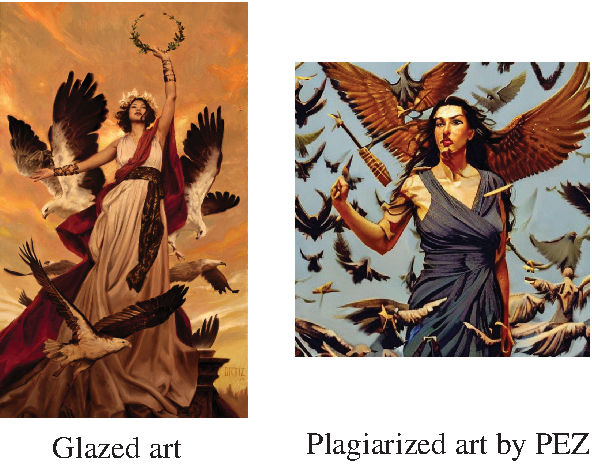
\includegraphics[width=0.90\columnwidth]{plots/counter/marx-counter.pdf}
  \vspace{-0.1in}
  \caption{Glazed image and generated image from PEZ mimicry method. The
    original image is {\em Musa Victoriosa}, a new painting created by Karla
    Ortiz to be the first artwork to be released publicly under \system{} protection.}
  \label{fig:marx-attack}
\end{figure}

\begin{figure}[t]
  \centering
  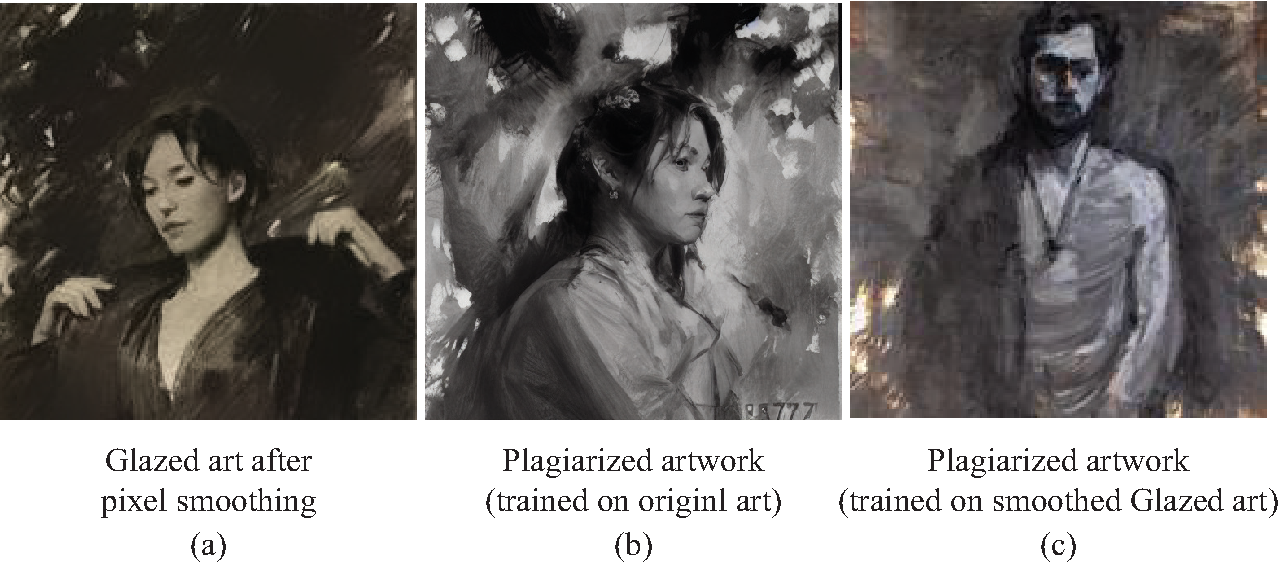
\includegraphics[width=0.90\columnwidth]{plots/counter/smoother.pdf}
  \vspace{-0.1in}
  \caption{ (a) Smoothed artwork by applying pixel smoother on Glazed
    artwork, (b) plagiarized artwork generated by training on original
    (unprotected) artwork, and (c) plagiarized artwork generated by training
    on Glazed artwork that was later pixel-smoothed.} 
  \label{fig:smooth-attack}
\end{figure}

Finally, while we have not yet observed any successful attacks against \system{},
we are continuously exploring design improvements to further enhance
robustness against potential future countermeasures.

%\vspace{-0.1in}
\section*{Acknowledgements} We thank our anonymous reviewers and shepherd for
their insightful feedback. We also thank Karla Ortiz, Lyndsey Gallant, Nathan
Fowkes, Kim Van Deun, Jon Lam, Eveline Fr\"ohlich, Edit Ballai, Kat Loveland and many
other artists, without whom this project would not be possible. This work is
supported in part by NSF grants CNS-2241303, CNS-1949650, and the DARPA GARD
program.  Opinions, findings, and conclusions or recommendations expressed in
this material are those of the authors and do not necessarily reflect the
views of any funding agencies.

